\section{User guide}
\label{sec:userguide}

\subsection{Before starting}
First, to create a ePNS file, the Eclipse runtime workbench should already be started. In it, the user should create an empty project so that it is later possible to group together all related files (PNML document, Geometry file, etc). An empty project can be created by selecting "File > New > Project > General > Project". Once this is done, there should be an empty folder in the Project explorer view.

\subsection{Petri net editor}
\index{ePNS Petri net}
\index{editors!Petri net}
\label{sec:userguide:petrinet}
\writer{Juan}

\subsubsection{Creating a new ePNS Petri net}
\label{sec:userguide:petrinet:create}
\index{ePNS Petri net!creation}
The creation of a Petri net file in an Eclipse runtime workbench will be detailed in this section. In this file the user will create the Petri net he/she would like to simulate and visualize.

Once the project has been created, the user can create a new Petri net file. To do so, he must right click on the project folder in the Project explorer view and select "New > Other > ePNK > PNML Document" \index{PNML Document} or do this via the "File" menu. The file creation wizard should have opened in a new window in Eclipse where a parent folder and a name for the Petri net file can be selected. The parent folder for the file can be chosen from the existing folders in the Eclipse environment (it is here one can select the empty project previously created to start grouping together all the files for the simulation). Any name can be given to the file as long as the \textit{.pnml} extension is kept. Once these two options have been adjusted, the file can be created by clicking on the "Finish" button.

Now that the file is created, some initial changes should be made in order to allow the edition of the Petri net. First, an ePNS Petri net document has to be created in the file. To do this, the recently created .pnml file should be opened and a child should be added to the "Petri Net Doc" by selecting the "New Child > Petri net (ePNS Petri net)" option in its right-click pop-up menu. \index{ePNS Petri net} Once the ePNS Petri net is created, a page should be added to it as a child by right clicking on it ("PetriNet") and selecting "New Child > Page".

\index{editors!validation}
One can now begin the edition of the Petri net (as described in the following sections). Once the editing process is completed, the Petri net has to be validated to check any errors that may have come up during said edition (e.g. conflicts with Arc Identies). This can be done by right-clicking on  the root element in the tree editor and selecting the "Validate" option.

\subsubsection{Adding items to the Petri net: Places, Transitions, Arcs, Tokens}
\label{sec:userguide:petrinet:add}
\index{ePNS Petri net!elements}
This section describes the addition of elements to a Petri net page previously created (see \ref{sec:userguide:petrinet:create}). These elements are the ones that describe the Petri net and it is from them that the simulation is inferred. This whole creation process can be done through a graphical editor that is shown by double clicking on the previously created page (see \ref{sec:userguide:petrinet:create}).

Three types of elements (nodes, arcs and labels, where tokens are a specific case of the latter) can be added to the Petri net, each of them in a different way.
\begin{itemize}
\index{ePNS Petri net!elements!node} \index{ePNS Petri net!elements!place} \index{ePNS Petri net!elements!transition}
\item The nodes of the Petri net can be either places or transitions, but they are all inserted in the same way. In the graphical editor the desired component must be selected by clicking on its corresponding icon in the \textit{Palette} shown on the right-hand side of the screen. After this, clicking on the canvas will insert a component of the selected type.
\index{ePNS Petri net!elements!arc}
\item The arcs of the Petri net connect nodes in the Petri net\footnote{Please note that arcs can only connect two different types of nodes between them.}. This can be done in the graphical editor there is an icon for arcs in the aforementioned Palette. Selecting it will enable the user to input arcs, which can be done by clicking on a node (this will be the arc's source 
\index{ePNS Petri net!elements!arc!source}) and dragging the mouse over to another node (this will be the arc's target 
\index{ePNS Petri net!elements!arc!target}).
\index{ePNS Petri net!elements!token}
\item The tokens of the Petri net are added to the places that have been previously created. The graphical editor presents the tokens as labels: to add a token to a place, create a label on the canvas (this can be done by clicking on the Label icon in the \textit{Palette} and clicking on the canvas) and link it to the place as a token (linking can be done by clicking on the outbound arrow that the label presents will selected and dragging it on to the place or by clicking on the Link Label icon in the \textit{Palette} and clicking on the label and the place; the label will represent a token if the \textit{Token} option is selected in the pop-up menu that appears when linking the label to the place).
\end{itemize}

\subsubsection{Setting some characteristics}
\label{sec:userguide:petrinet:setup}
\index{ePNS Petri net!attributes}
Once the components of the desired Petri net have been added to the page, some editing is in order
to customize it. This editing is done through the Properties view (shown when clicking on an element
and selecting the "Show Properties View" in its right-click pop-up menu) or through the graphical
editor, depending on the charasteristic to set. The different attributes that can be changed for
each element shall now be described:
\index{ePNS Petri net!attributes!Interactive Input} \index{ePNS Petri net!attributes!Geometry Label} \index{ePNS Petri net!attributes!Animations}
\begin{description}
\label{sec:userguide:petrinet:setup:places}
  \item[Places] have main four attributes that can be modified: \textit{Id},
  \textit{interactiveInput}, \textit{Geometry Label} and \textit{Animation Label}. The Id is used to
  identify the place; interactiveInput indicates if the place is an inputPlace, \index{input place}
  i.e. a place into which tokens can be inserted from the simulation, through a mouse click; the
  Geometry Label is used to associate the place with a geometry element (See
  \ref{sec:userguide:geometry:elements}); and the Animations label contains the animations
  associated to the place (See \ref{sec:userguide:animations}). The Id and interactiveInput feature
  can be edited in the Properties View by selecting each one and modifying its value (either writing
  on the text box or selecting from the options provided, depending on each attribute). The Geometry
  and Animations Labels must be added through the graphical editor by selecting a \textit{Label} in
  the Palette and clicking on the canvas. To associate it to a specific place, the user can either
  click on the label and drag the outgoing arrow that will appear over to the place, or click on the
  Link Label icon in the \textit{Palette} and click then on the label and the place. When releasing
  the click button, the \textit{Geometry Label} or \textit{Animation Label} option should be
  selected from the pop-up menu that is shown. The text in the label can be edited by selecting the
  label and writing the desired animation (See section \ref{sec:userguide:animations:types}).
  Besides, if the place is an Input Place, a fifth attribute can be added: Input Place Appearance
  Label, a Label that indicates the appearance of the tokens externally inserted in that place. This
  label is created in the same way as Geometry or Animation Labels.
 \item[Tokens in Places] can have an \textit{appearance} associated to them, which indicates their
 graphical representation in the simulation. This characteristic is set by editing the text of the
 Token Label (this text can be anything, although later it must coincide with the name of an
 appearance created in the Appearance Editor; for more information see
 \ref{sec:userguide:appearance}).
 
 \item[Transitions] have the attribute \textit{Id}, which can be modified in the Properties View.
 \label{sec:userguide:petrinet:token:appearance} \index{ePNS Petri net!attributes!Appearance}  
  
\index{ePNS Petri net!attributes!identity}
  \item[Arcs] have one attribute, \textit{identity}, which can be edited through the Properties View. It is used to determine the trajectory of the tokens when a 
  transition is fired.
\end{description}

\subsubsection{Animations}
\index{animations}
\label{sec:userguide:animations}
Introducing animations into a Petri net model will allow the user to define the way in which the behaviour of the Petri net is represented in the final graphical visualization. The animations will be applied to Tokens when they move into a Place, so it will be in these last elements where Animations shall be edited. This is done by writing on an \textit{Animation Label} in the Petri net editor (see \ref{sec:userguide:petrinet:setup:places} for more details). Here the different types of Animations and their parameters shall be described, as well as the syntax that must be used to properly insert them into the Petri net. 
\index{animations!move}

\label{sec:userguide:animations:types}
The animations that can be used for the visual representation of a Petri net are the following:

\begin{description}
  \item[Move:] written as \textit{move(speed)}, this Animation will move graphical representation of the Token (see \ref{sec:userguide:petrinet:token:appearance}) at a certain \textit{speed} along the track assigned (as a Geometry Label) to the Place. \index{animations!move}
  \item[Wait:] written as \textit{wait(time)}, the 3D Engine managing the visualization will simply do nothing to the Token's representation for the specified amount of \textit{time} (in miliseconds). \index{animations!wait}
  \item[Show:] written as \textit{show(label)}, it shows the object referenced by the \textit{label} (see \ref{sec:userguide:appearance} in the position of the 2D plane connected (as a Geometry Label) to the Place.
  \item[Hide:] written as \textit{hide()}, it hides from view the object that is in the position of the 2D plane connected (as a Geometry Label) to the Place. \index{animations!hide}
  \item[Sequence:] this is a special type of Animation composed of two or more of the previously described Animations. It must be written following the scheme \textit{animation;animation;...}, i.e., as animations separated by semicolons. \index{animations!sequence}
\end{description}

%%%%%%%%%% Geometry Editor %%%%%%%%%%%
\subsection{Geometry Editor}
\writer{George, Jerome}
\index{geometry}
\index{editors!geometry}
\label{sec:userguide:geometry}

%%% New geometry file
\subsubsection{Creating a new Geometry file}
\label{sec:userguide:geometry:create}
This section will explain how a Geometry file can be created using the Eclipse runtime workbench.

A Geometry file can be created with the use of wizards. Like all Eclipse creation wizards, the one
that is needed for Geometry file creation can be accessed via the \textit{New} menu, either by
clicking on the "File" menu of the menu bar or by right-clicking on the Explorer of the workbench.
The user then has to choose "Other..." for moving to the next "Select a wizard" dialog. What has
been done so far could be also achieved by pressing "Ctrl+N", a shortcut that makes things simpler.
Now, the user is ready to finally choose the type of file he wants to create. In the "Select a
wizard" dialog he can either type the string "Geometry Diagram" - note that is not case sensitive -
or he can find this option under "Examples", in the same dialog.

In the dialog "Create Geometry Diagram" the user can change the name given to the graphical editor. In the last step, by selecting "Next" he can optionally change the name of the tree editor as well. This task is completed by clicking on "Finish". Now the user should be able to see the new project place in the runtime workbench Explorer.

%%% General stuff about geometry elements
\subsubsection{Geometry elements: TrackPosition, Track, SimplePosition}
\label{sec:userguide:geometry:elements}
\index{geometry!track} \index{geometry!simple position} \index{geometry!track position}
There are two editors with which the user can create a Geometry, the tree editor and the graphical editor. Nevertheless we will see later that the graphical editor is safer and easier to use, so the tree editor shouln't be used in most of the cases. These editors can be populated with some elements, namely \textit{Tracks}, \textit{TrackPosition} and \textit{SimplePosition}. 

A \textbf{Track} represents the path that a track-bound object will move on. A \textbf{TrackPosition} denotes either the starting point of a Track or its ending point. As as far as the Track element is concerned, it should be linked with two TrackPosition so that the Geometry is valid. The two following sections (\ref{sec:userguide:geometry:tree} and \ref{sec:userguide:geometry:graphical}) will explain how to add such objects, describing the editors in details. Last but not least, a \textbf{SimplePosition} represents a point on the Geometry of a particular interest. On this point a static object, a traffic light for instance, can be put to control the behavior of the track bound moving object that follows the path that a Track elements has defined. A SimplePosition can be placed anywhere in the Geometry. 

%%% Howto use the tree editor
\subsubsection{The tree editor}
\label{sec:userguide:geometry:tree}
The tree editor is the one of the two editors that becomes available after the creation of a new Geometry file. The file-format for this editor is recognized by the ".geometry" suffix. Double-clicking on a file of that type will start the tree editor. The user can also edit this type of file by clicking on the little arrow on the left of the filename ending with a ".geometry" while he is inside the Explorer. With this editor the user can create and delete elements of the Geometry. However it is advisable to use the graphical editor for that purpose instead, since it is easier to use and the user gets an immediate picture of the changes he/she is doing to the Geometry. Indeed, the use of the graphical editor for creation and deletion of Geometry elements is safer, since inconsistencies might emerge otherwise between the two editors. This is the reason why this document does not elaborate more on how to create or delete Geometry elements in the tree editor. Figure \ref{fig:geo_tree_editor} shows an overview of the tree editor editing a Geometry file.

\begin{figure}[htp]
\begin{center}
  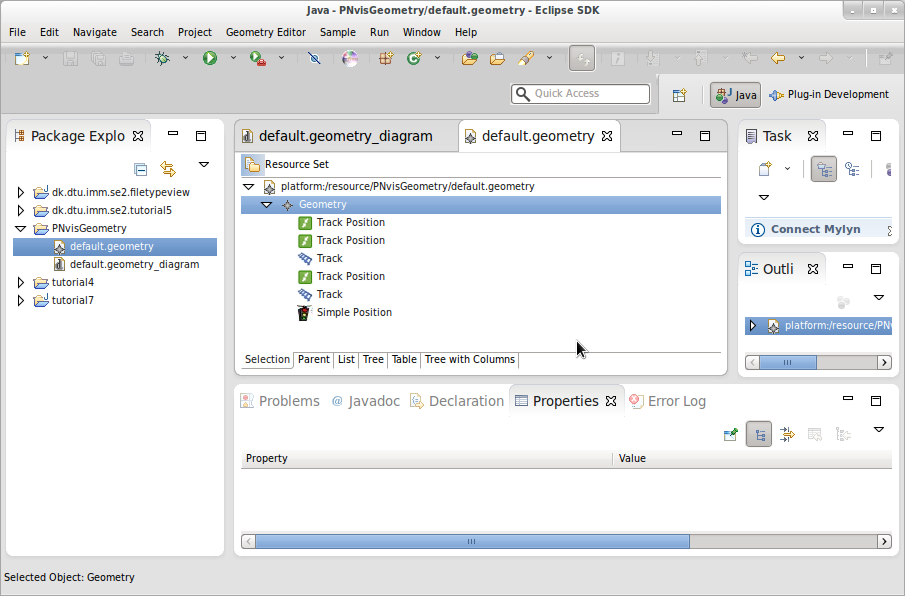
\includegraphics[width=10.0cm]{image/geo_tree_editor.png}
  \caption{Overview of the tree editor for a Geometry file}
  \label{fig:geo_tree_editor}
\end{center}
\end{figure}

\index{editors!validation}
An important action that the user can perform using the tree editor is to validate the Geometry he has built. This can be done by right-clicking on the top element of the tree editor. Then, in the pop-up menu he has to select "Validate". If the validation succeeds the user will be notified with a message on the emerged dialog. In case of validation failure the same dialog will give the user the user the chance to investigate failure related messages by clicking on the "Details" button. 

%%% Howto use the graphical editor
\subsubsection{The graphical editor}
\label{sec:userguide:geometry:graphical}
The graphical editor is the second editor that becomes available after the creation of a new Geometry file. It should be used to edit these Geometry files as it is safer and easier to use than the tree editor. The file-format for this second editor can be found thanks to the ".geometry\_diagram" suffix. To open this editor the easiest way is to double-click on a file with that suffix and that previously created inside the Explorer (see section \ref{sec:userguide:geometry:create}). Figure \ref{fig:geometry_overview} shows an overview of the graphical editor with an open Geometry file.

\begin{figure}[htp]
\begin{center}
  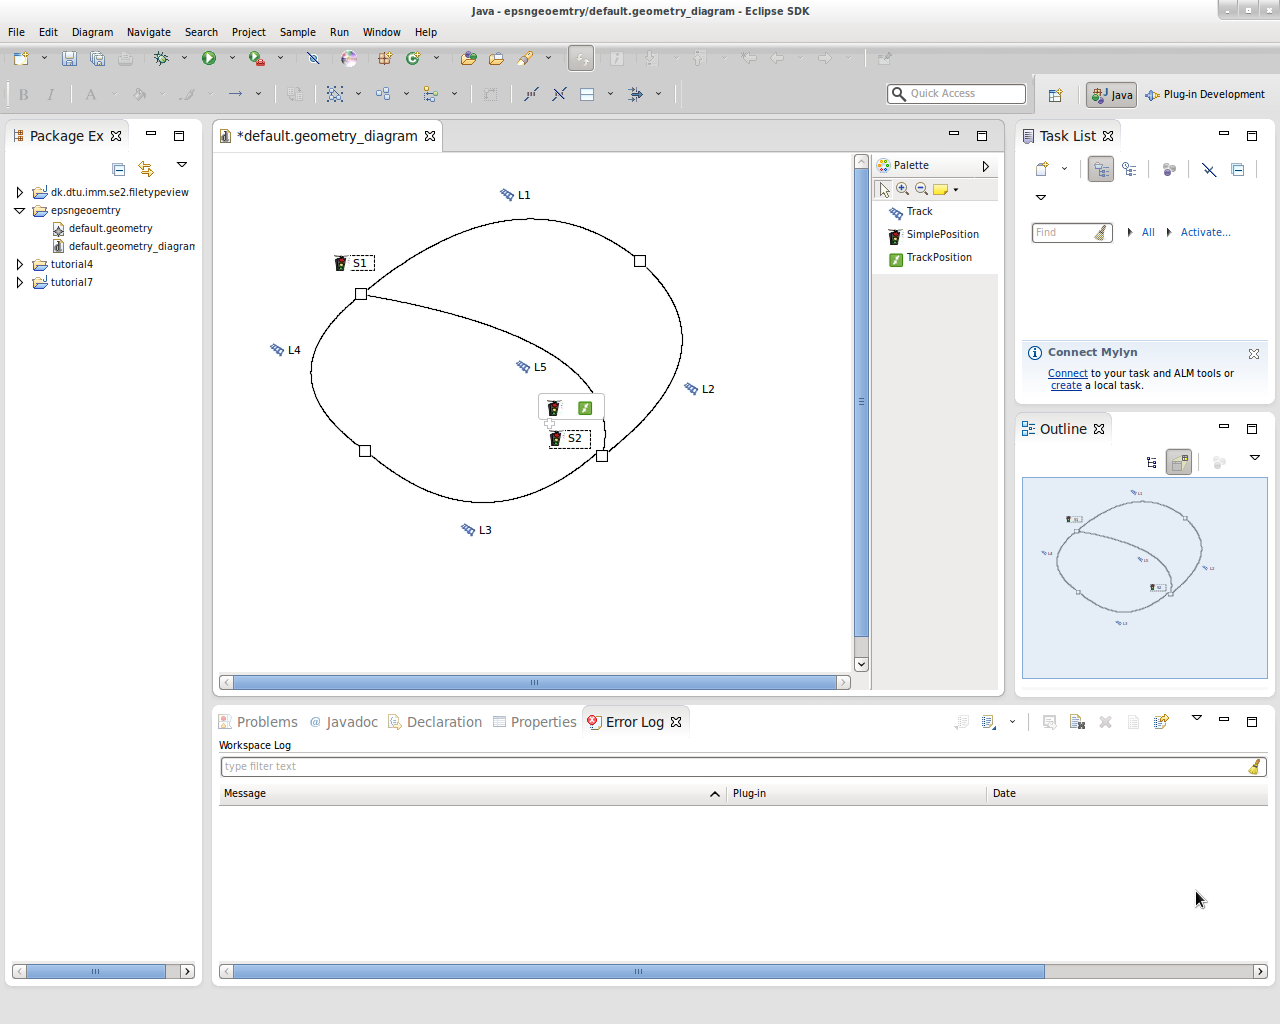
\includegraphics[width=10.0cm]{image/geometry_general.png}
  \caption{Overview of the graphical editor for a Geometry file}
  \label{fig:geometry_overview}
\end{center}
\end{figure}

On the right-side of the editor, the \textit{palette} or tool bar of the graphical editor can be seen. This allows the user to create Geometry objects. We will come to that part a little bit later. At the top, the \textit{tab} of this page can also be seen, displaying the name of the document. 

To create Geometry objects the user needs to click on the element he wants to create inside the \textit{palette} and drop it where he wants it to be inside the canvas. There are three different objects he can create with the graphical editor for Geometry files : a TrackPosition, a Track, and a SimplePosition. He can have a look at section \ref{sec:userguide:geometry:elements} to understand in which case each element should be used. It must be noted that the reader cannot create a Track if he/she has not previously created at least one TrackPositions. 

%Finally the user can undo and redo actions by using the shortcuts "CTRL+Z" (undo) or "CTRL+SHIFT+Z" (redo) or by clicking on the corresponding entries in the "Edit" menu. Indeed the user can save his document by hitting "CTRL+S" or "File" -> "Save".% // Ekkart said : useless...

%%% Set characteristics
\subsubsection{Setting some characteristics}
\label{sec:userguide:geometry:characteristics}
Ultimetaly, the reader must set some characteristics of the Geometry objects in order to make the simulation running with appropriate visuals. These characteristics can be inspected at the Properties View  for each object. If this view is not visible in the workbench, go to the menu "Windows" -> "Show View" -> "Other..." and inside "General" double-click on the "Properties" (view). This view will now display additional properties for each object selected. Some of this properties are already defined, such as the starting point and ending point of a Track, while others need to be defined, for instance the AppearanceLabel of a Track.

\label{sec:userguide:geometry:appearance}
To configure correctly the Geometry file the user must define some of these additional properties. For the Track object and the SimplePosition object the user will have to define an AppearanceLabel that is a label refering to some appearance defined in the Appearance Editor (see section \ref{sec:userguide:appearance:new}). This can be done by clicking on the object once created and double-clicking in the right-zone corresponding to the AppearanceLabel inside the properties view, then writing some text using the keyboard. For the TrackPosition object the user will not have to define anything more.

Finally, the user can change the Label of some Tracks and SimplePositions by clicking on the name-label inside the graphical editor and start typing the new name or by selecting the object and changing the value of the field Label inside the properties view.
%%%%%%%%%%%%%%%%%%%%%%%%%%%%%%%%%%%%%

\subsection{Appearance Editor}
\index{appearance}
\index{editors!appearance}
\label{sec:userguide:appearance}
\writer{Pablo}

\subsubsection{Creating a new Appearance file}
\label{sec:userguide:appearance:create}
The creation of an Appearance file is done by selecting "New > Other > Example EMF Model Creation Wizards > Appearance Model" and clicking on the "Next" button. The next window allows both the selection the parent folder for the file and the edition of the name of said file (maintaining the \textit{.appearance} extension). After editing these two things and clicking on the "Next" button, the option "ePNS Appearance Model" must be chosen as a Model Object. Clicking on "Finish" will create the Appearance file.

\subsubsection{Adding items to the Appearance: Model3D, Shape3D, Texture, SurfaceColor}
\index{appearance!Model3D} \index{appearance!Shape3D} \index{appearance!Texture} \index{appearance!SurfaceColor}
\label{sec:userguide:appearance:add}
Once there is an Appearance file created (see above), elements can be added to it. To do it the Appearance file must be open and its root node expanded. In said node will be a node "ePNS Appearance Model", where right clicking permits the addition of an element to the Appearance file by means of the "New Child" option. Here the user can choose between four elements: Model3D, Shape3D, Texture and SurfaceColor.
\subsubsection{Setting some characteristics}
\index{appearance!attributes}
\label{sec:userguide:appearance:edit}
Simply having an Appearance file created and adding elements to it will not suffice, for these elements need to refer to something that describes the Appearance, as well as having a name to associate them to the components of the Petri net. The attributes of each element that can be edited are here presented, each of them editable in the Properties view of the selected element:
\index{appearance!Model3D} \index{appearance!Shape3D} \index{appearance!Texture} \index{appearance!SurfaceColor}
\begin{itemize}
  \item All elements have a \textit{label} attribute that gives each one a name and will later allow the connection to the components of the Petri net.
  \item Both \textbf{Model3D} and \textbf{Shape3D} objects have: a \textit{scale} to make them bigger or smaller; three rotation values (\textit{xRotation}, \textit{yRotation} and \textit{zRotation}) to rotate them; and an \textit{elevation} attribute to raise the shape.
  \item \textbf{Model3D} also has a \textit{file} attribute, which is a reference to a file where the desired Appearance is described. This file must be located in the Ecplipse workbench.
  \item A \textbf{Shape3D} also allows the modification of its \textit{type} attribute. This attribute grants the user the choice to select the object's Appearance among a series of predefined shapes (cube, sphere...).
  \item A \textbf{Texture} has a \textit{file} attribute analogous to the \textit{file} attribute in the Model3D (again, this file must be located in the Ecplipse workbench).
  \item Finally, the \textbf{SurfaceColor} will have a \textit{Color}, which can be chosen from the 13 predefined colours.
\end{itemize}

Shapes (Model3D and Shape3D elements) can also have a surface (Texture or SurfaceColor). To add this, right-click on the desired shape and select "New Child" and "Texture" or "SurfaceColor". The properties of the selected surface can be changed again using the Properties View.

\subsubsection{Adding appearances to Tokens, Tracks and Simple Positions}
To add appearances to Tokens, Tracks and SimplePositions, one must have created both a Petri net and a corresponing Geometry. See \ref{sec:userguide:geometry:appearance} and \ref{sec:userguide:petrinet:token:appearance} for information on how to do this.

\subsection{Configuration Editor}
\label{sec:userguide:configuration}
\index{configuration}
\index{editors!configuration}
\writer{Marius}

\subsubsection{Creating a new Configuration file}
\label{sec:userguide:configuration:new}
This subsection gives details on the creation and proper setting of a Configuration file.
With all the Geometry, Appearance and PNML resources created, a Configuration file is needed, to link them all together. The Configurator gives the user the possibility to use, for example, the same Geometry and PNML files, but with a different Appearance file.
To create a new Configurator file, the user must go to File -> New -> Other, and from Example EMF Model Creation Wizards select Configurator model and click Next. From there, he should select a parent folder, give the new file a name and click on Finish. 

\subsubsection{Loading resources and setting Configurator properties}
To load the resources and set the Configurator properties, the user should first open the Configurator file. In the tree-view, it can be seen that the file contains a Configurator object. Here, the Appearance, Geometry and PNML resources need to be loaded. This is done by right-clicking in the active window and selecting "Load Resource". Then, after having selected "Browse Workspace", the Appearance file created as in step \ref{sec:userguide:configuration:new} must be selected and click Ok. The same process must be repeated for the Geometry and PNML files. The order in which these files are loaded is not important. They can also be loaded all at once. 

To set the configurator properties, the user has to click on the Configurator and in the property view, in the Appearance field, he should click on the Value field and select "ePNS Appearance Model" from the dropdown menu. Similarly, for the Geometry property, "epns.geometry" must be loaded, and for Petri net, "Petri Net Doc" must be selected. Another property that the user should set is the Default Track Width. Its default value is 1.0, but a bigger value is recommended, so that the tracks can be easily distinguished.

\subsubsection{Starting a simulation}
With the Geometry, Appearance and PNML resources loaded and selected in the configurator, to start
the simulator, the user has to right-click on the Configurator object and select the \textit{Start
simulator} menu item. A new window will appear, in which the simulation would run. More details can
be found in section \ref{sec:userguide:simulator}.

\subsection{Simulator}
\label{sec:userguide:simulator}
\index{simulator}
\writer{Ruxandra}

\subsubsection{Starting the simulator}

The Simulator can be started by clicking on the Start Simulator option after right clicking on the Configuration 
item from the .configurator file, after loading and linking the geometry, the appearance and the Petri net files, 
as described in \ref{sec:userguide:configuration}.

\subsubsection{Controlling the simulation: Play/pause/stop}
After starting the simulator, a new window like the one shown in figure \ref{fig:simulator} will be displayed.
The simulation can be played by pressing the Start Button on the left side of the window. 

The simulation can be stopped at any time. By stopping it, the simulation will return to the initial state. The 
simulation can then be played again by pressing the Start button.

At any time, the simulation can be paused, by pressing the Pause button. It can then be resumed by pressing the Resume button, which will
replace the Pause button after a pause.

\begin{figure}[htp]
\begin{center}
  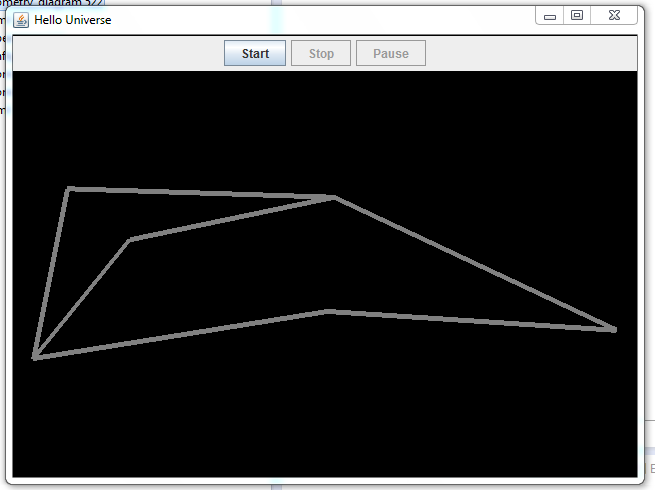
\includegraphics[width=10.0cm]{image/simulator.png}
  \caption{Simulator interface}
  \label{fig:simulator}
\end{center}
\end{figure}

\subsubsection{User Interaction}
\index{input place}
The user can interact with the animation by using the input places. The interactivity for a place is set in the 
pnml file as described in section \ref{sec:userguide:petrinet:setup}. If a place is an input place, it usually has associated
an appearance as a Single Object and is placed on a SimplePosition (see section \ref{sec:userguide:geometry:elements} for details) , rather than a track. 
In this way, the user can click on the object visually associated to the place and insert a token into the place.
Another way the user can interact with the simulation is by changing the view point. There are 3 ways to move that camera: scroll to zoom in/out,
right click and drag to pan the camera and left click and drag to rotate the camera.



